\documentclass[14pt, aspectratio=169]{beamer}
\usetheme{Warsaw}
\usecolortheme{seahorse}
\usepackage{graphicx} % Required for inserting images
\usepackage{wrapfig}
\usepackage{comment}
\setbeamertemplate{navigation symbols}{}

\title{Examining Muon Scattering Tomography for Imaging Nuclear Materials}
\author{Aditya Patwardhan}
\institute{Institute for Computing in Research}
\date{August 2023}

\begin{document}

\maketitle

\begin{frame}{Table of Contents}
    \begin{enumerate}
        \item<2-> Muons
        \item<3-> Muon Scattering Tomography
        \item<4-> Implementing the Simulation
        \item<5-> Results
        \item<6-> Putting it Together
    \end{enumerate}
\end{frame}
\begin{frame}{}
    \large \textbf{Muons}
\end{frame}
\begin{frame}{}
    \centering
    \begin{figure}
        \centering
        \includegraphics<1->[width=0.5\textwidth,height=0.75\textheight]{images/muoncascade.jpg}
        \caption{Cosmic ray muons \cite{muonimage}}
    \end{figure}
    
\end{frame}

\begin{frame}{}
    \large \textbf{Muon Scattering Tomography}
\end{frame}
\begin{frame}{Muon Scattering Tomography}
    \centering
    \only<1> {
        \begin{figure}
            \centering
            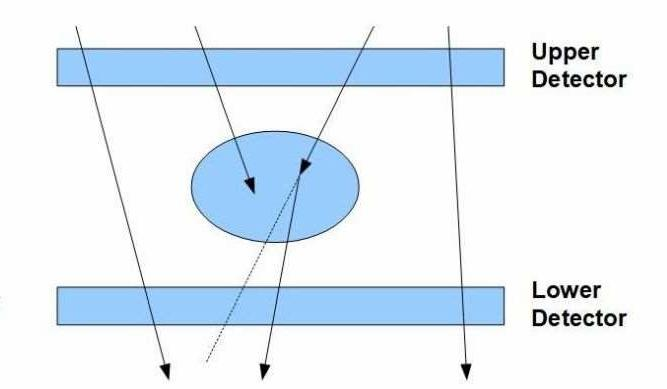
\includegraphics[scale = 0.4]{images/mst principle.jpg}
            \caption{Muon scattering tomography \cite{international2022iaea}}
        \end{figure}
        
    }
    \only<2> {
        \large The greater the atomic number, the greater the scattering angle
    }
    \only<3>{
        \begin{figure}
            \centering
            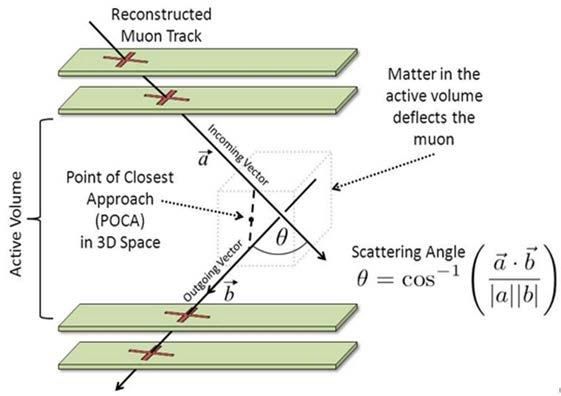
\includegraphics[scale=0.4]{images/scattering angle.jpg}
            \caption{Obtaining scattering angle from PoCA algorithm \cite{international2022iaea}}
        \end{figure}
        
    }
\end{frame}

\begin{frame}{}
    \large \textbf{Implementing The Simulation}
\end{frame}

\begin{frame}{Programming the Simulation}
    \centering
    \only<2> {
        \begin{figure}
            \centering
            
\includegraphics[scale=1]{images/geant4logo.png}
            \caption{Geant4 - CERN's particle physics library. \cite{geant4logo}}
        \end{figure}
    }
    \only<3> {
        \large \text{But not in C++}
    }
    \only<4> {
        \begin{figure}
            \centering
            \includegraphics<4->[scale=0.2]{images/pybind11-logo.png}
            \caption{Pybind11 - use C++ with Python \cite{pybind11}}
        \end{figure}
    }
    
\end{frame}

\begin{frame}{Processing the Data}
        
    \only<2> {
        \centering
        \begin{figure}
            \centering
            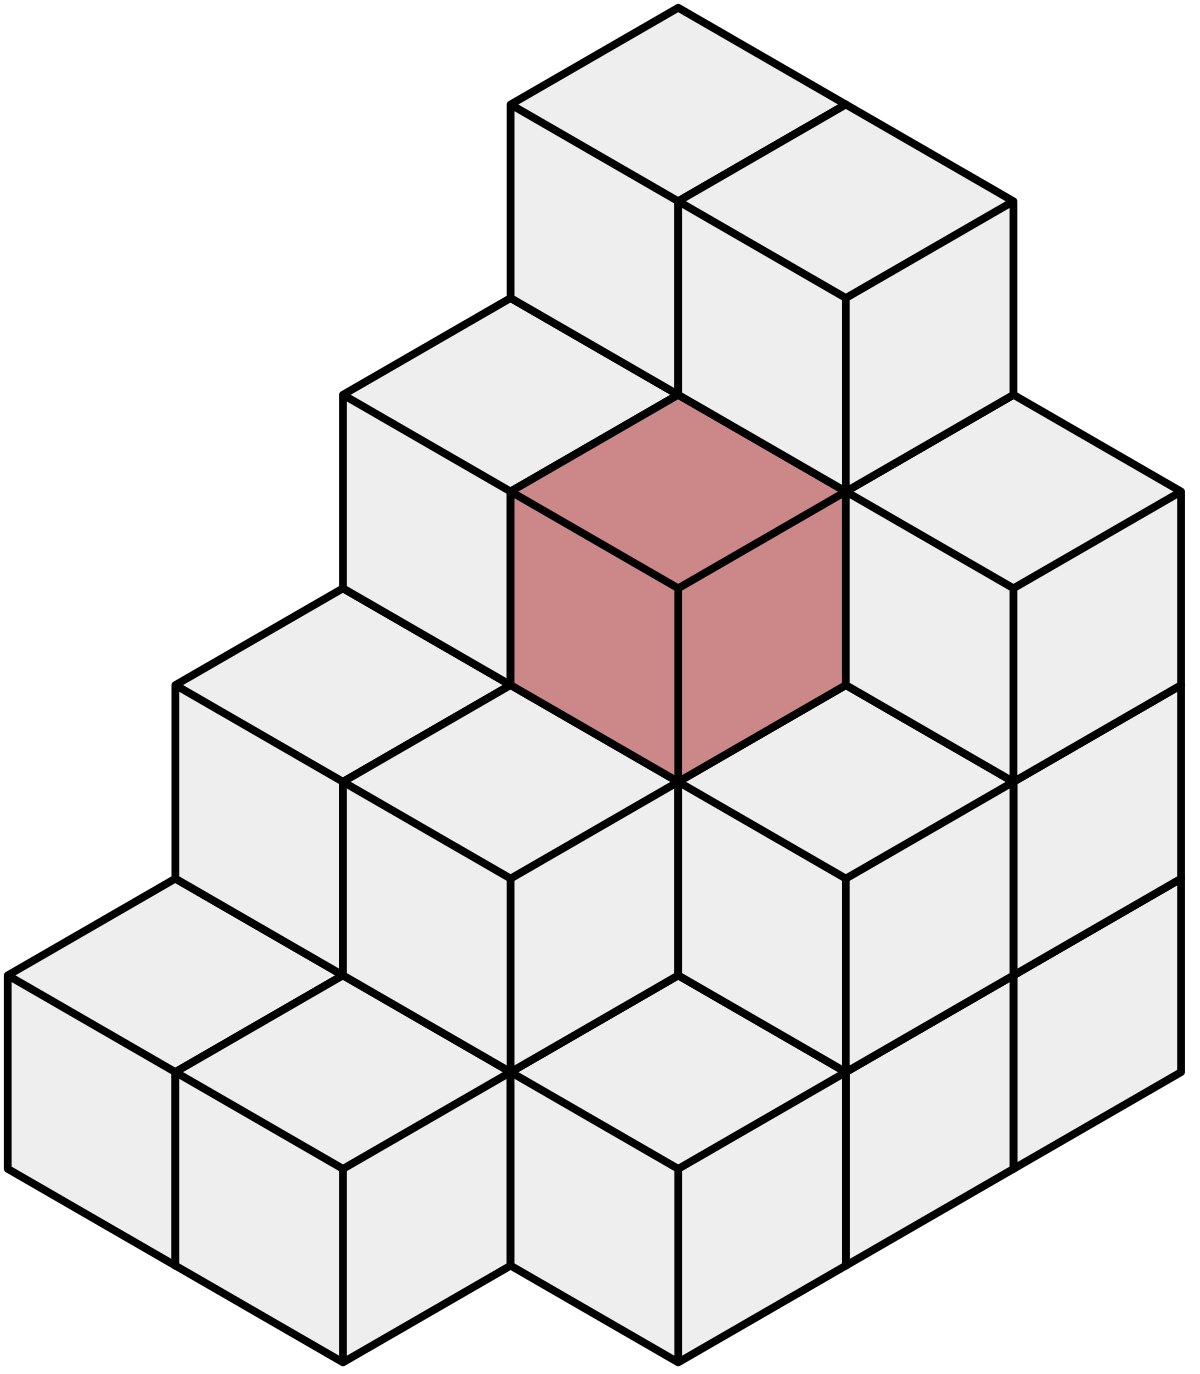
\includegraphics[scale=0.1]{images/Voxels.svg.png}
            \caption{Voxels \cite{voxel}}
            \label{fig:enter-label}
        \end{figure}
        
    }
    \only<3-> {
        \begin{itemize}[<+->]
            \item<4-> Only scattering angles \(>\) 1.5°
            \item<5-> Filtered based on density and location
            \begin{equation}
                F(n, s) = C \cdot n \cdot s^3
            \end{equation}
            \begin{itemize}
                \item C = filtering coefficient
                \item n = number of voxels
                \item s = side length of voxel
            \end{itemize}
        \end{itemize}
    }

\end{frame}


\begin{frame}{}
    \large \textbf{Results}
\end{frame}

\begin{frame}{Evaluation method}
    \begin{itemize}
        \item<2-> Accuracy score
        \begin{equation}
            A(C, S) = 100 \cdot \frac{2 \cdot |C \cap S|}{|C| + |S|}
        \end{equation}
        \begin{itemize}
            \item C = Correct set of voxels
            \item S = Simulated set of voxels
        \end{itemize}
        \item<3-> Voxel side lengths are factors of material cube side length
    \end{itemize}
\end{frame}

\begin{frame}{Scattering Angles}
    \begin{wrapfigure}{l}{\textwidth}
    %\centering
    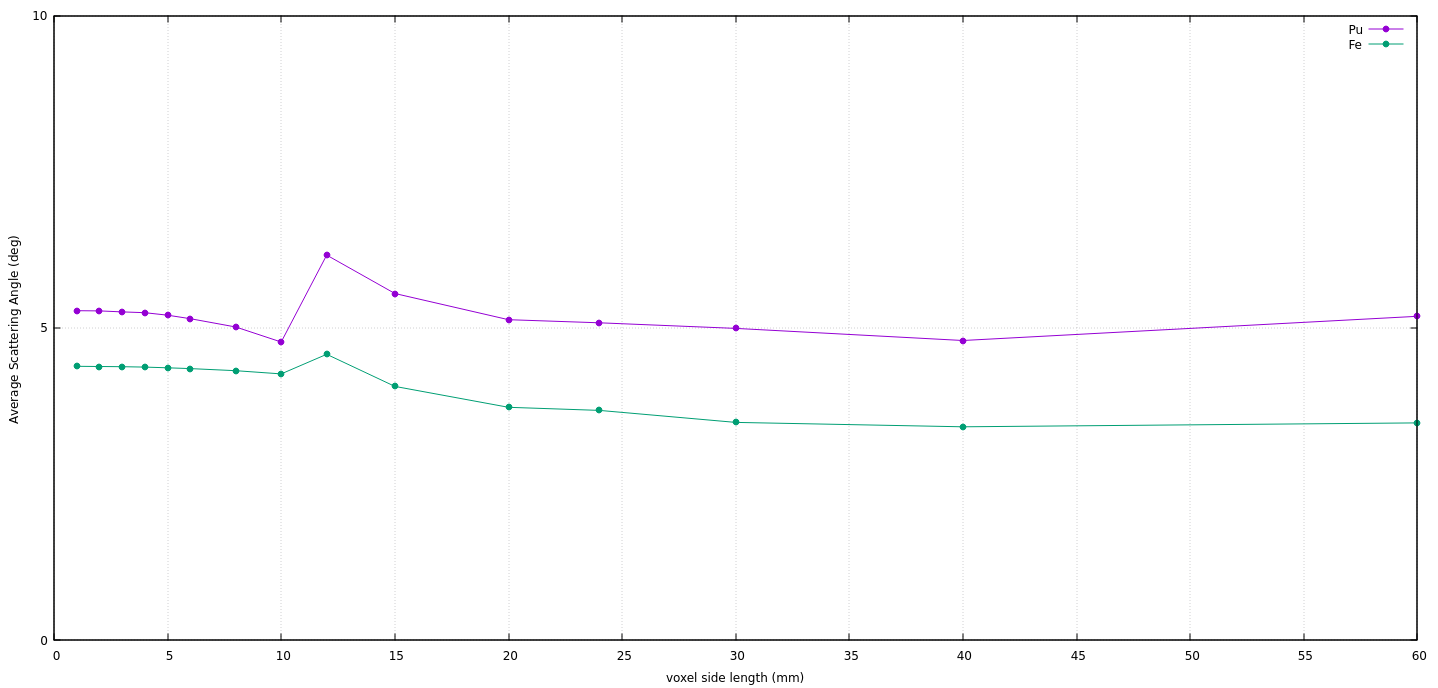
\includegraphics[width=\textwidth]{images/smaller avg scattering angle vs voxel side length.png}
        \caption{Average Scattering Angle (°) vs Voxel Side Length (mm)}
    \end{wrapfigure}
\end{frame}

\begin{frame}{Voxel Detection Accuracy}
    \begin{wrapfigure}{l}{\textwidth}
    %\centering
        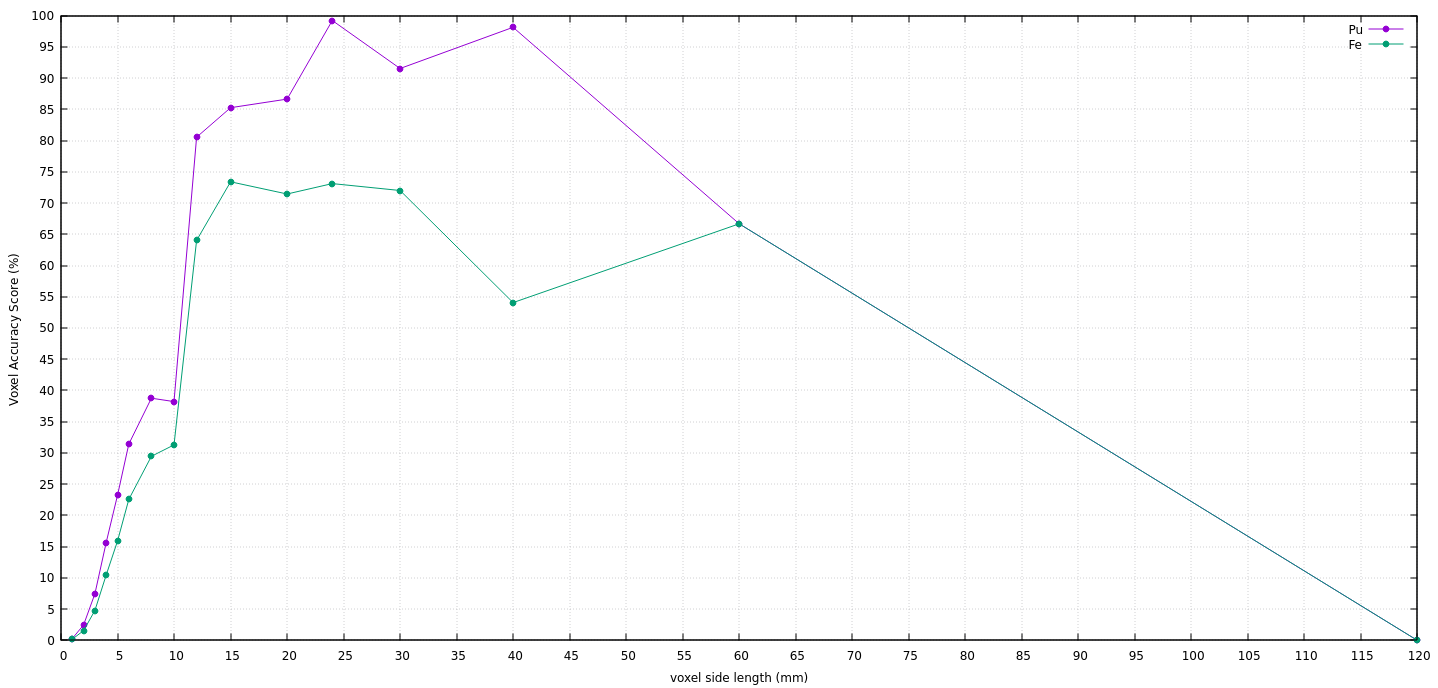
\includegraphics[width=\textwidth]{images/smaller voxel accuracy score vs side len.png}
            \caption{Voxel Accuracy Score (\(\%\)) vs Voxel Side Length (mm)}
    \end{wrapfigure}
\end{frame}

\begin{frame}{Images}
   \begin{wrapfigure}{l}{\textwidth}
    %\centering
        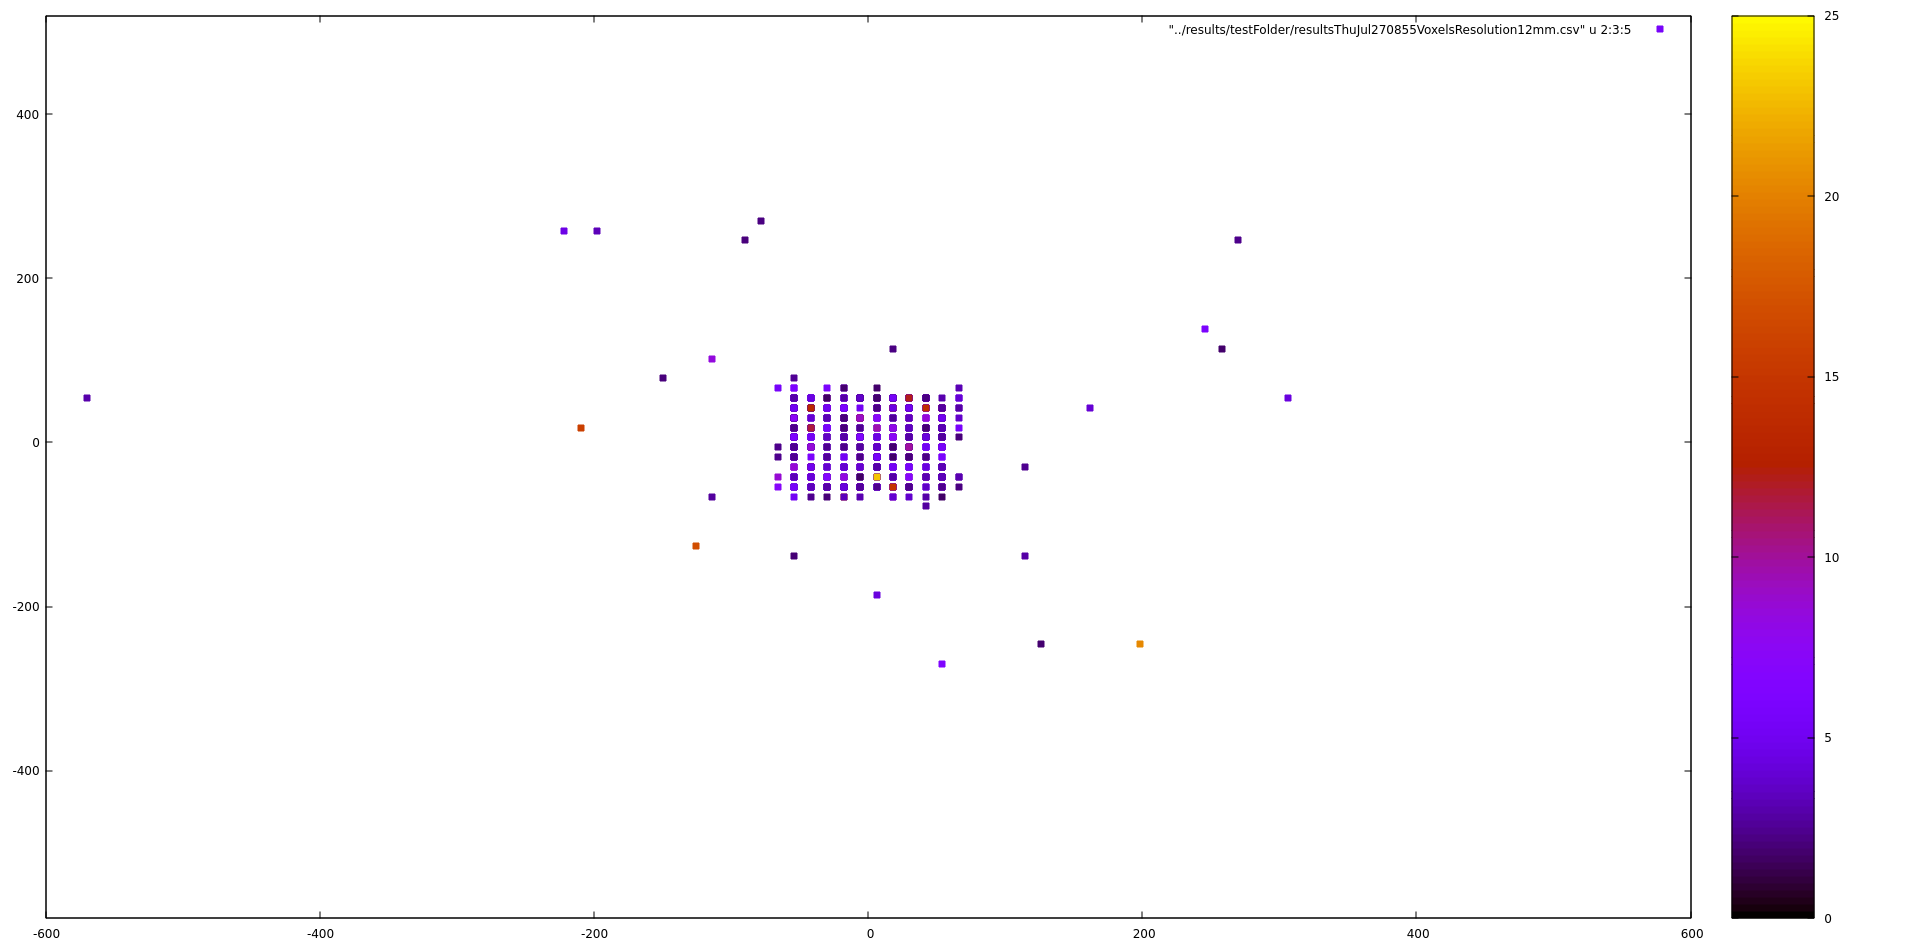
\includegraphics[width=\textwidth]{images/12mm res iron.png}
            \caption{Fe Voxelized image 2D}
    \end{wrapfigure}
    
\end{frame}
\begin{frame}
    \begin{wrapfigure}{l}{\textwidth}
    %\centering
        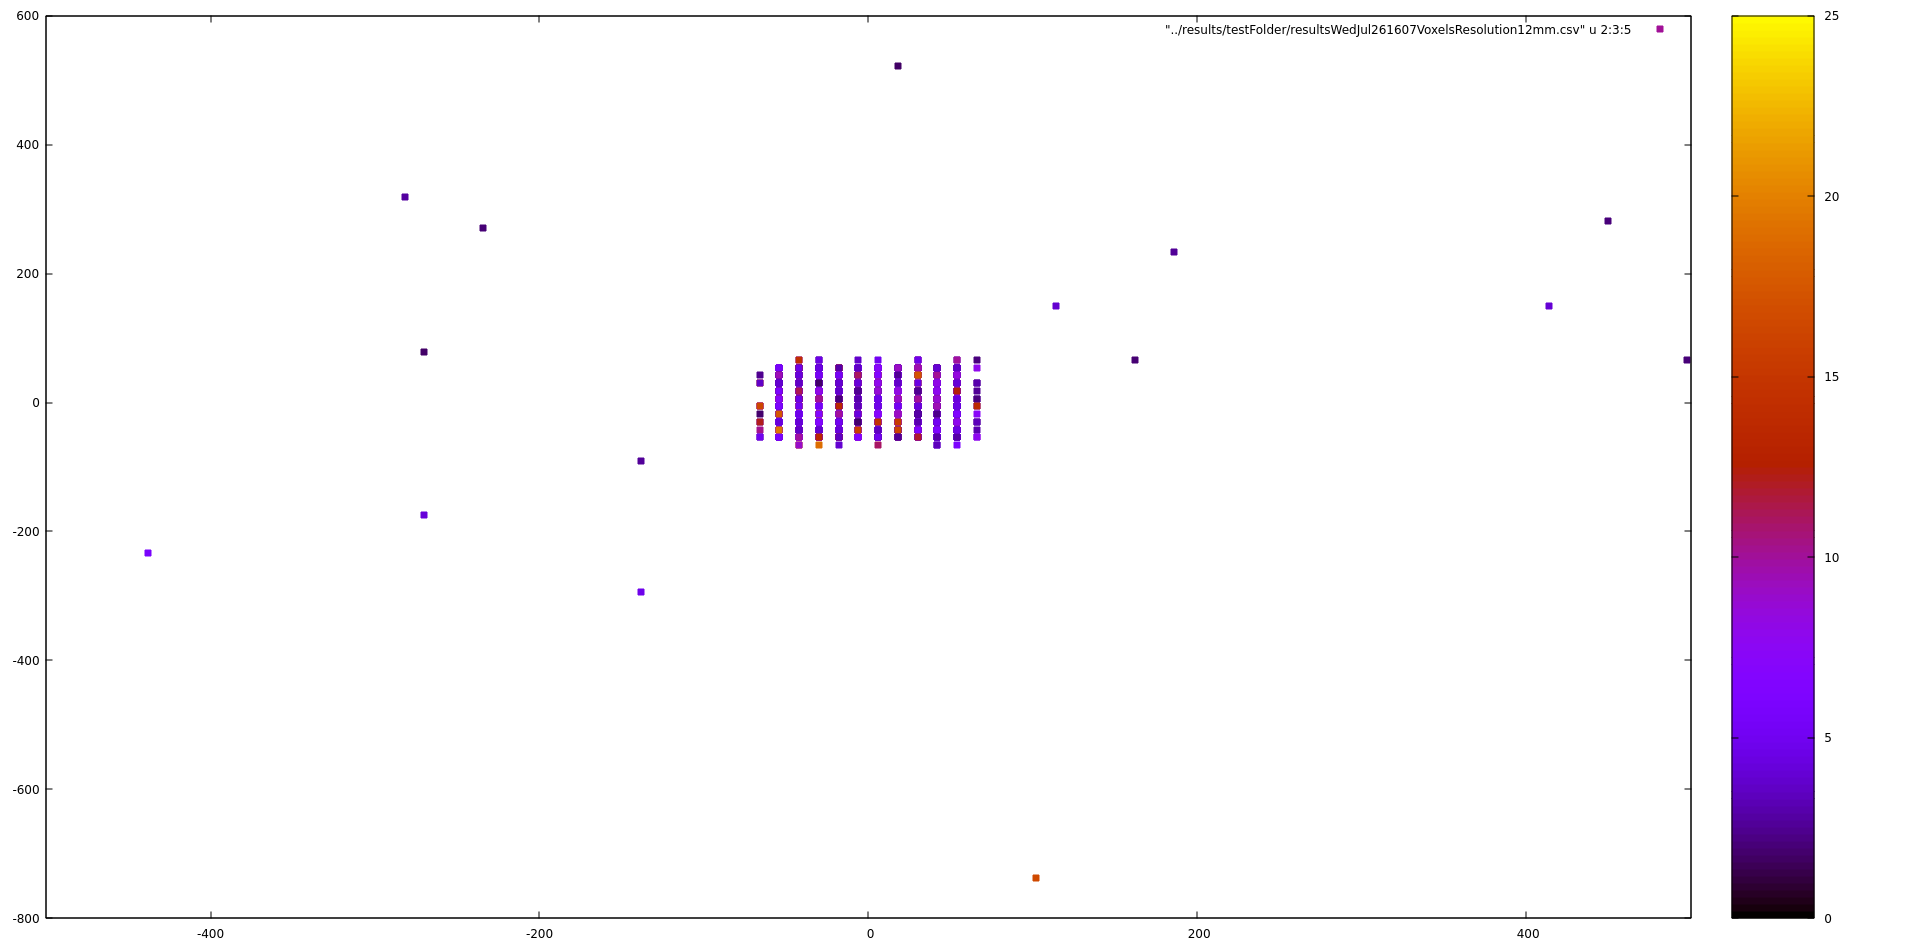
\includegraphics[width=\textwidth]{images/12mm res plutonium.png}
            \caption{Pu Voxelized image 2D}
    \end{wrapfigure}
\end{frame}

\begin{frame}{}
    \large \textbf{Putting it Together}
\end{frame}

\begin{frame}{Putting it Together}
    \begin{itemize}
        \item<1-> Evaluating the system
        \item<2-> Calibrating for accuracy
        \item<3-> Future research
    \end{itemize}

\end{frame}


\begin{frame}{}
    \large \textbf{Questions?}
\end{frame}


\begin{frame}{}
    \large \textbf{Sources}
\end{frame}
\begin{frame}[allowframebreaks]{Sources}
    \bibliographystyle{ieeetr}
    \bibliography{citation}
\end{frame}
\end{document}
